  	
  %-----------------------------------------------------------------%
  %   Architecture et explication détaillé de l'implémentation
  %-----------------------------------------------------------------%
  \chapter{Architecture du programme}
  
  \section{Lancement du programme}
  Des options de lancement ont été rajouté au programme , leurs utilisations sont disponible en annexe \ref{annexe:usage}
  

  \section{Système de rendu}
  Le programme est découpé en classes afin d'abstraire les appels à la bibliothèque OpenGL. La figure \ref{fig:uml_scene} représente le diagramme des classes qui forment l'abstraction principale du programme.
  Les classes relatives à la génération, l'affichage de la planète et l'utilisation du CDLOD sont strockés dans le dossier
  PlanetTech.
  
  \begin{figure}
  \centering
  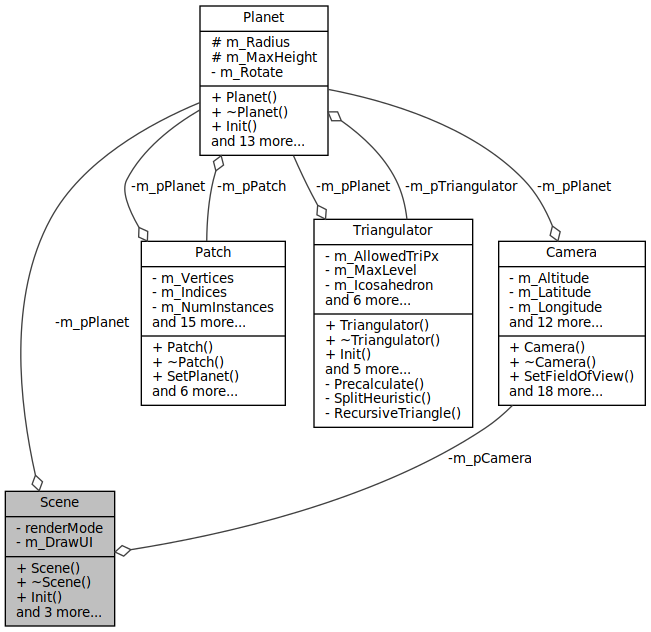
\includegraphics[width=10cm]{img/uml_scene.png}
  \caption{Diagramme de classe de Planet}
  \label{fig:uml_scene}
  \end{figure}

  La classe Scene est la classe centrale du programme, elle permet
  d'initialiser et de créer la planète. Scene gère les paramètres
  principaux du programme à travers les entrées clavier d'InputManager.
  Ces paramètres sont le nombre de niveaux de détail, le mode d'affichage
  (texture + maillage, maillage uniquement, texture uniquement). Scene
  gère aussi l'affichage des informations comme le compteur d'images par
  seconde ou le nombre de sommets actuellement affiché.
  
  La classe Planet représente la sphère à afficher. Ses classes filles
  (voir figure \ref{fig:inh_planet} spécialisent le type de planète
  à afficher, ce sont elles qui définissent la taille de la sphère,
  sa texture et sa carte de hauteur.\\
  
  \begin{figure}
  \centering
  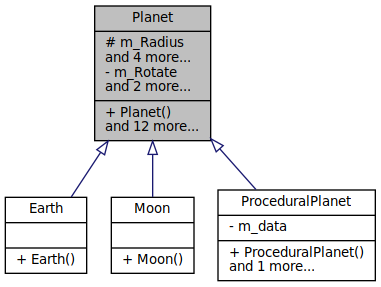
\includegraphics[width=10cm]{img/planet_inh.png}
  \caption{Diagramme d'héritage de Planet}
  \label{fig:inh_planet}
  \end{figure}
  
  %\begin{figure}
  %centering
  %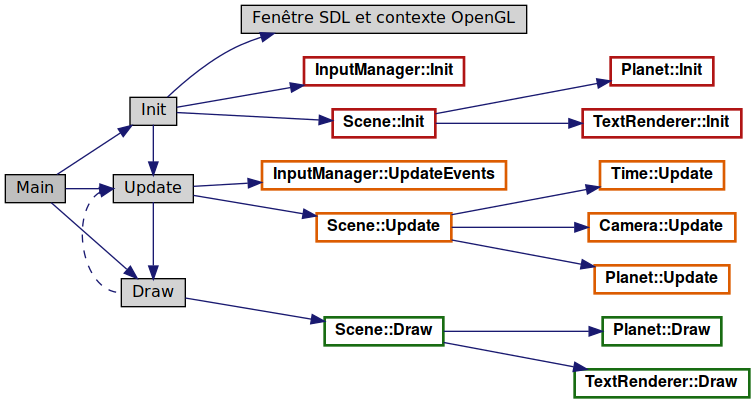
\includegraphics[width=10cm]{img/plan_exec.png}
  %\caption{Plan}
  %\label{fig:triangulator}
  %\end{figure}
 
  La figure \ref{fig:plan} représente le graphe simplifié de
  l'exécution du programme. L'étape d'initialisation se fait une seule
  fois au début du programme, et les étapes de mise à jour et d'affichage
  se répètent tout le long de l'exécution.
  
\section{Heightmap}
  
  Le programme utilise un \emph{quadtree} pour générer les différents niveaux de détail. 
  Ensuite une nouvelle hauteur est appliquée à ce point pour le déplacer. 
  Cependant, le \emph{quadtree} ne stocke pas la hauteur du sommet. Cette dernière
  est enregistrée dans une texture 2d et est envoyée à la carte graphique. 
  Chaque pixel de la texture représente donc une valeur codée sur un nombre flottant entre -1 et 1.
  La texture récupérée par la carte graphique, est plaquée sur le maillage de la sphère et la hauteur du sommet
  est déduite de l'interpolation des texels de la texture sur le maillage.
    %définir texel
  %définir interpolation ?
  
  \section{Triangulator}
  La classe Triangulator permet de générer le \emph{quadtree} utilisé pour le système de niveau de détail.
  Un objet Frustum est utilisé pour décider si un triangle de l'arbre est ou non dans le cône 
  de vision de la caméra. Le diagramme de classes présenté en figure \ref{fig:plan} présente la classe
  Triangulator. Les différents composants seront analysés plus loin dans le chapitre implémentation.
  
  \section{Patch}
  La classe Patch récupère les triangles envoyés par Triangulator, et les subdivise (beaucoup) tout en appliquant l'algorithme de morphing. La subdivision n'est calculée qu'une seule fois à l'initialisation, tous les triangles sont ensuite subdivisés de la même façon. Ce mécanisme est possible grâce au mécanisme de EBO/VBO d'openGL. C'est excellent en matière de performance. Cela permet d'atteindre un grand nombre de triangle sans que ceux-ci n'apparaissent directement dans la récursion du CPU. Cela diminue aussi la taille des transferts.
  Le morphing permet non seulement d'adoucir les différences entre les niveaux de détails et mais aussi et surtout d'éliminer les trous.
  
  
  \begin{figure}
  \centering
  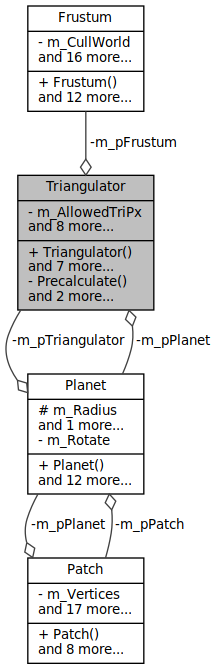
\includegraphics[width=5cm]{img/tri_class2.png}
  \caption{Diagramme de classe de Triangulator}
  \label{fig:plan}
  \end{figure}
  
  \section{Frustum}
  La classe Frustum permet de faire la différence entre un triangle dans le champ, un triangle partiellement dans le champ, et un triangle hors champ. Le Frustum est utilisé par la classe Triangulator lors de la construction du maillage.\\
  
  Cette classe a pour but d'éliminer les triangles qui ne sont pas visibles. Cette opération appelée \textit{culling} accélère la génération en supprimant des noeuds de récursion, diminue la taille de transfère entre CPU/GPU, et diminue le nombre de triangles à dessiner dans la carte graphique.
  
  
 \newpage %pour placer les images correctement
 